\section{Sound waves}
Sound waves are pressure (density) waves in a compressible medium.

\begin{align}
p&=p_0+\tilde{p}, \quad\tilde{p}\ll p_0\\
\rho&=\rho_0+\tilde{\rho}, \quad\tilde{\rho}\ll\rho_0
\end{align}
Equation of state:
\begin{equation}
\rho=\rho_0(1+\kappa(p-p_0))
\end{equation}
The parameter $\kappa$ is called compressibility.
\begin{equation}
\tilde{\rho} = \rho_0\kappa\tilde{p}
\end{equation}

Assumption: small velocities.
\begin{equation}
\vec{u}=0+\tilde{\vec{u}}.
\end{equation}

Euler equation without friction:
\begin{equation}
\rho\left(\pdiff{\vec{u}}{t}+\left(\vec{u}\cdot\vec{\nabla}\right)\vec{u}\right)=-\vec{\nabla}p
\end{equation}

\begin{equation}
(\rho_0 + \tilde{\rho})\pdiff{\tilde{\vec{u}}}{t}+(\rho_0+\tilde{\rho})\left(\tilde{\vec{u}}\cdot\vec{\nabla}\right)\tilde{\vec{u}} = -\vec{\nabla}\tilde{p}
\end{equation}

\begin{equation}\label{eq:sound-1}
\pdiff{\tilde{\vec{u}}}{t}=-\frac{1}{\rho_0}\vec{\nabla}\tilde{p}
\end{equation}

Equation of continuity:
\begin{align}
\pdiff{\rho}{t}+\vec{\nabla}\left(\rho\vec{u}\right)&=0\\
\leadsto
\pdiff{\tilde{\rho}}{t}+\vec{\nabla}\left((\rho_0+\tilde{\rho})\tilde{\vec{u}}\right) &= 0\\
\leadsto
\pdiff{\tilde{\rho}}{t}+\rho_0\vec{\nabla}\tilde{\vec{u}}&=0\label{eq:sound-2}
\end{align}
Divergence of \eqref{eq:sound-1}:
\begin{equation}
\vec{\nabla}\pdiff{\tilde{\vec{u}}}{t}=-\frac{1}{\rho_0}\vec{\nabla}\cdot\vec{\nabla}\tilde{p}
\end{equation}
Time derivative of \eqref{eq:sound-2}:
\begin{equation}
\ppdiff{\tilde{\rho}}{t}+\rho_0\pdiff{}{t}\vec{\nabla}\tilde{\vec{u}}=0
\end{equation}

\begin{align}
\Delta\tilde{p} &= -\rho_0\vec{\nabla}\pdiff{\vec{u}}{t} \\
&= \ppdiff{\tilde{\rho}}{t}
\end{align}

Wave equation:
\begin{equation}
\Delta\tilde{p} = \rho_0\kappa\ppdiff{\tilde{p}}{t} = \frac{1}{c^2}\ppdiff{\tilde{p}}{t}
\end{equation}

In 1+1 dimensions:
\begin{equation}
\ppdiff{\tilde{p}}{x} = \frac{1}{c^2}\ppdiff{\tilde{p}}{t}
\end{equation}

Plane-wave solution:
\begin{equation}
\tilde{p} = A_p\cos(x-ct)
\end{equation}

Here $c=\frac{1}{\sqrt{\rho_o\kappa}}$ is the speed of sound. Examples:
\begin{align}
c_\mathrm{air} &= \SI{340}{m/s} \\
c_\mathrm{water} &= \SI{1500}{m/s}
\end{align}

"Density wave":
\begin{equation}
\ppdiff{\tilde{\rho}}{x} = \frac{1}{c^2}\ppdiff{\tilde{\rho}}{t} \Rightarrow \tilde{\rho}=A_\rho\cos(x-ct)
\end{equation}

Longitudinal "velocity wave":
\begin{align}
\pdiff{\tilde{u}_x}{t} &= -\frac{1}{\rho_0}\pdiff{\tilde{p}}{x}= \frac{A_p}{\rho_0}\sin(x-ct) \\
\leadsto
\tilde{u}_x &= \frac{A_p}{\rho_0c}\cos(x-ct) = A_u\cos(x-ct)
\end{align}

Validity of approximation, which has neglected small quadratic terms in the Euler equation:
\begin{align}
\frac{|\left(\vec{u}\cdot\vec{\nabla}\right)\vec{u}|}{|\pdiff{\vec{u}}{t}|} = \frac{|v_x\pdiff{v_x}{x}|}{|\pdiff{v_x}{t}|} \approx \frac{A_u^2}{A_uc} = \frac{A_u}{c} \approx \frac{|\vec{u}|}{c}
\end{align}
Typical velocity oscillations are much smaller than the speed of sound:
\begin{equation}
\frac{|\vec{u}|}{c} \ll 1.
\end{equation}
\begin{framed}
\textbf{Example:} loudspeaker
\begin{equation}
f=100-\SI{2000}{Hz} \Rightarrow f_\mathrm{typical} = \SI{1000}{Hz}
\end{equation}
Amplitude of membrane displacement $\Delta x \approx \SI{1}{mm}$

\begin{align}
\Delta u &\approx \frac{\Delta x}{\Delta t/2} \approx \frac{\SI{2e-3}{m}}{\SI{e-3}{s}} \\
 &= \SI{2}{m/s} \ll c_\mathrm{air}
\end{align}
\end{framed}

\newpage
\subsection{Outlook: shock waves}
\begin{figure}[!h]
    \centering
    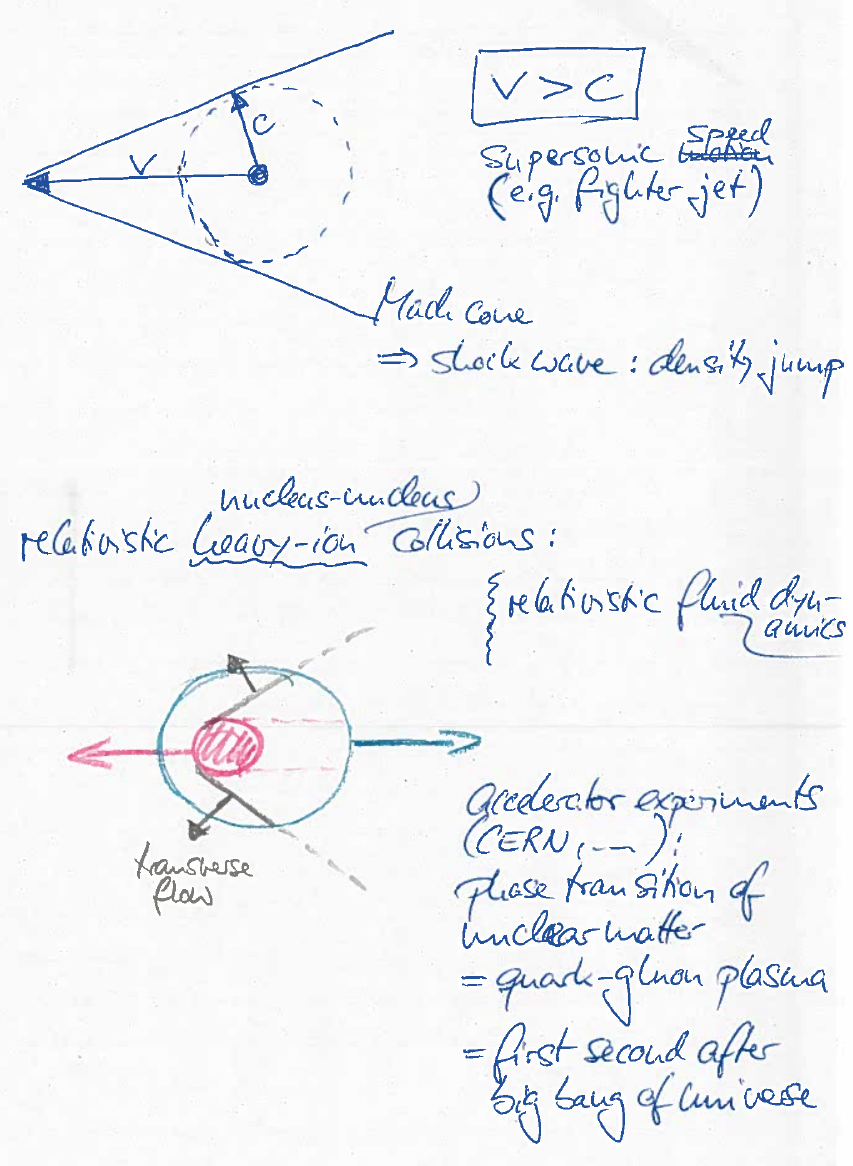
\includegraphics[width=\textwidth]{week6/shock-waves}\\
    \caption{Sketches of shock waves.}
    \label{fig:shock-waves}
\end{figure}